% Options for packages loaded elsewhere
\PassOptionsToPackage{unicode}{hyperref}
\PassOptionsToPackage{hyphens}{url}
%
\documentclass[
]{report}
\usepackage{lmodern}
\usepackage{amssymb,amsmath}
\usepackage{ifxetex,ifluatex}
\ifnum 0\ifxetex 1\fi\ifluatex 1\fi=0 % if pdftex
  \usepackage[T1]{fontenc}
  \usepackage[utf8]{inputenc}
  \usepackage{textcomp} % provide euro and other symbols
\else % if luatex or xetex
  \usepackage{unicode-math}
  \defaultfontfeatures{Scale=MatchLowercase}
  \defaultfontfeatures[\rmfamily]{Ligatures=TeX,Scale=1}
\fi
% Use upquote if available, for straight quotes in verbatim environments
\IfFileExists{upquote.sty}{\usepackage{upquote}}{}
\IfFileExists{microtype.sty}{% use microtype if available
  \usepackage[]{microtype}
  \UseMicrotypeSet[protrusion]{basicmath} % disable protrusion for tt fonts
}{}
\makeatletter
\@ifundefined{KOMAClassName}{% if non-KOMA class
  \IfFileExists{parskip.sty}{%
    \usepackage{parskip}
  }{% else
    \setlength{\parindent}{0pt}
    \setlength{\parskip}{6pt plus 2pt minus 1pt}}
}{% if KOMA class
  \KOMAoptions{parskip=half}}
\makeatother
\usepackage{xcolor}
\IfFileExists{xurl.sty}{\usepackage{xurl}}{} % add URL line breaks if available
\IfFileExists{bookmark.sty}{\usepackage{bookmark}}{\usepackage{hyperref}}
\hypersetup{
  pdftitle={  STAT 216 Activity Coursepack},
  hidelinks,
  pdfcreator={LaTeX via pandoc}}
\urlstyle{same} % disable monospaced font for URLs
\usepackage{longtable,booktabs}
% Correct order of tables after \paragraph or \subparagraph
\usepackage{etoolbox}
\makeatletter
\patchcmd\longtable{\par}{\if@noskipsec\mbox{}\fi\par}{}{}
\makeatother
% Allow footnotes in longtable head/foot
\IfFileExists{footnotehyper.sty}{\usepackage{footnotehyper}}{\usepackage{footnote}}
\makesavenoteenv{longtable}
\usepackage{graphicx,grffile}
\makeatletter
\def\maxwidth{\ifdim\Gin@nat@width>\linewidth\linewidth\else\Gin@nat@width\fi}
\def\maxheight{\ifdim\Gin@nat@height>\textheight\textheight\else\Gin@nat@height\fi}
\makeatother
% Scale images if necessary, so that they will not overflow the page
% margins by default, and it is still possible to overwrite the defaults
% using explicit options in \includegraphics[width, height, ...]{}
\setkeys{Gin}{width=\maxwidth,height=\maxheight,keepaspectratio}
% Set default figure placement to htbp
\makeatletter
\def\fps@figure{htbp}
\makeatother
\setlength{\emergencystretch}{3em} % prevent overfull lines
\providecommand{\tightlist}{%
  \setlength{\itemsep}{0pt}\setlength{\parskip}{0pt}}
\setcounter{secnumdepth}{-\maxdimen} % remove section numbering
\usepackage{booktabs}
\usepackage{geometry}
\usepackage[none]{hyphenat}

\pagestyle{plain}

%%%% Set margins?... doesn't work
%\setlength{\topmargin}{-1cm}
%\addtolength{\evensidemargin}{-1cm}
%\addtolength{\oddsidemargin}{-1cm}
%\addtolength{\textheight}{1.8cm}
%\addtolength{\textwidth}{2cm}
\usepackage[]{natbib}
\bibliographystyle{plainnat}

\title{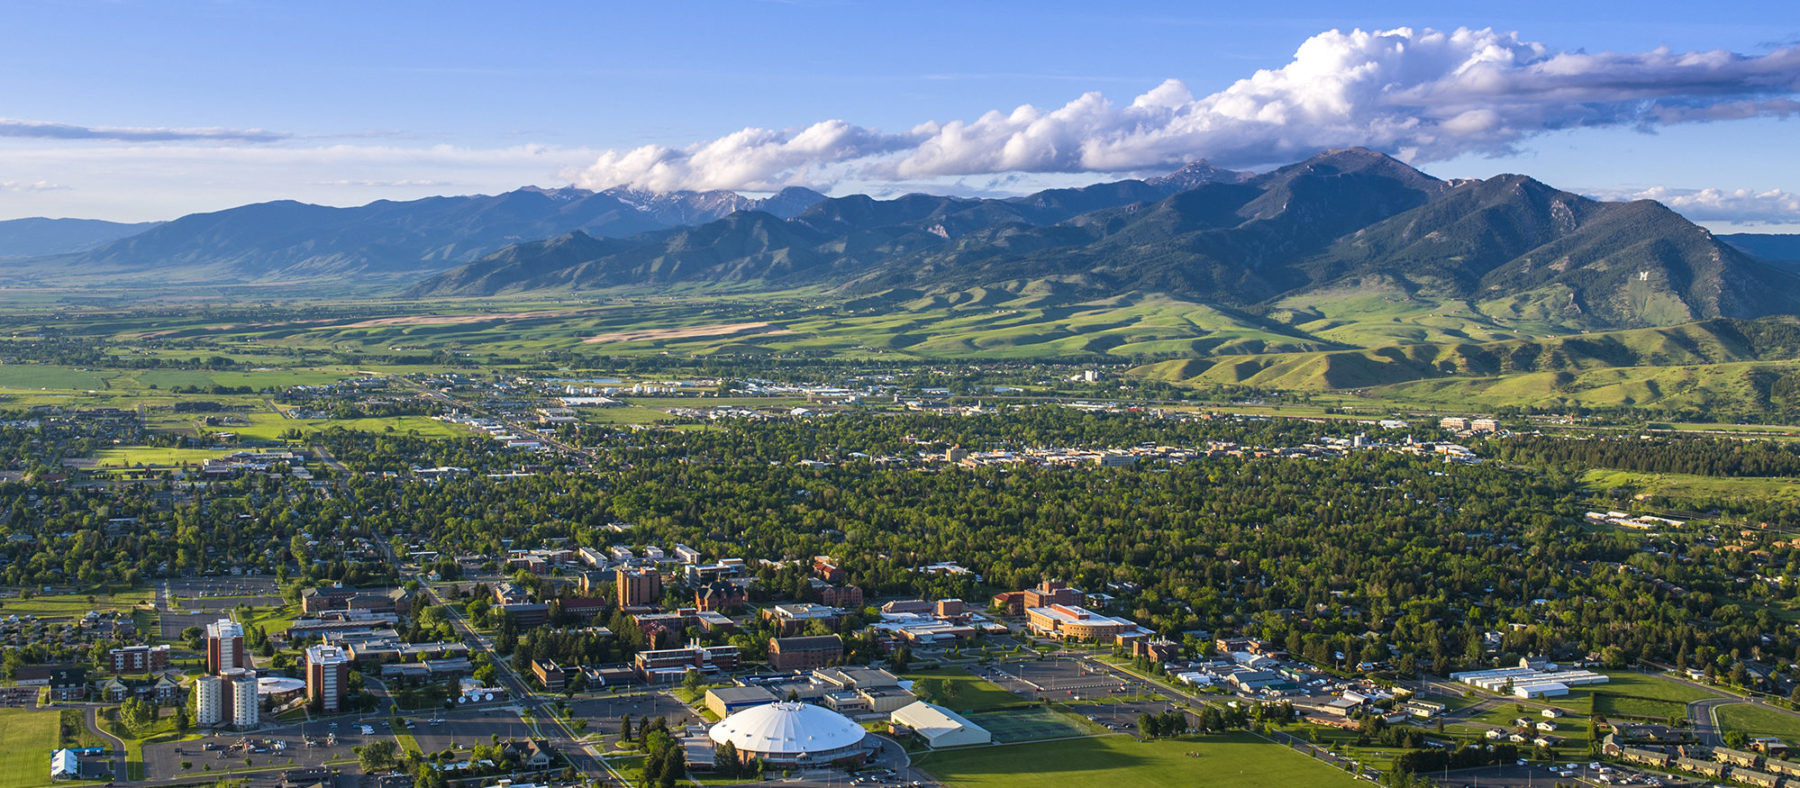
\includegraphics[width=5in,height=\textheight]{images/msu-campus.jpg}
\vspace{1cm}\\
STAT 216 Activity Coursepack}
\usepackage{etoolbox}
\makeatletter
\providecommand{\subtitle}[1]{% add subtitle to \maketitle
  \apptocmd{\@title}{\par {\large #1 \par}}{}{}
}
\makeatother
\subtitle{Fall 2020}
\author{}
\date{\vspace{-2.5em}}

\begin{document}
\maketitle

{
\setcounter{tocdepth}{0}
\tableofcontents
}
\hypertarget{preface}{%
\chapter{Preface}\label{preface}}

This coursepack accompanies the textbook for STAT 216: Introduction to Statistics at Montana State University. Each of the activities in this workbook is designed to target specific learning outcomes of the course, giving you practice with important statistical concepts in a group setting with instructor guidance. Bring this workbook with you to class each week, and take notes in the workbook as you would your own notes. A well-written complete workbook will provide an optimal study guide for exams!

\hypertarget{martian-alphabet-an-introduction-to-statistics}{%
\chapter{Martian Alphabet: An Introduction to Statistics}\label{martian-alphabet-an-introduction-to-statistics}}

\hypertarget{learning-outcomes}{%
\section{Learning Outcomes}\label{learning-outcomes}}

\begin{itemize}
\item
  Describe the statistical investigation process
\item
  Identify observational units, variables, and variable types in a statistical study
\end{itemize}

How well can humans distinguish one ``Martian'' letter from another? In today's activity, we'll find out. When shown the two Martian letters, kiki and bumba, write down whether you think bumba is on the left or the right.

\vspace{0.5in}

\hypertarget{steps-of-statistical-investigation}{%
\section{Steps of Statistical Investigation}\label{steps-of-statistical-investigation}}

The first step of any statistical investigation is to ask a research question. In this study the research question is: can we as a class read Martian? (we will refine this later on!). To answer any research question, we must design a study and collect data. (This will normally be provided for you in class.) For our question, the study consists of each student being presented with two Martian letters and asking which was bumba. Your responses will become our observed data that we will explore. To answer the research question we will simulate what \emph{could} have happened in our class given random chance, repeat that many times to understand the expected variability between different ``randomly guessing'' classes, then comparing our class's observed data to the simulation. This gives us an estimate of how often (or the probability of) our class's result would occur if we were all merely guessing, allowing us to determine if we as a class can in fact read Martian.

Let's explore the data.
\textbf{Observational units} or \textbf{cases} are the subjects data is collected on. In a data set the rows will represent a single observational unit.

\begin{enumerate}
\def\labelenumi{\arabic{enumi}.}
\tightlist
\item
  What are the observational units in this study?
\end{enumerate}

\vspace{0.5in}

\begin{enumerate}
\def\labelenumi{\arabic{enumi}.}
\setcounter{enumi}{1}
\tightlist
\item
  How many students are in class today? This is the sample size.
\end{enumerate}

\vspace{0.5in}

A \textbf{variable} is information collected or measured on each observational unit or case. We will look at two types of variables: \textbf{quantitative} and \textbf{categorical}. Each column in a data set will represent a different variable.

Quantitative variables are numerical measurements that can be discrete (whole, non-negative numbers) or continuous (any value within an interval). The number of students in a class would be a discrete variable as you can not have a partial student. GPA would be a continuous variable ranging from 0 to 4.0.

Categorical variables are data that are in groups or categories such as eye color, state of residency, or whether or not a student is considered in-state. Categorical variables with a natural ordering are considered ordinal variables while those without a natural ordering are considered a nominal variable. All variables will be treated as nominal for analysis.

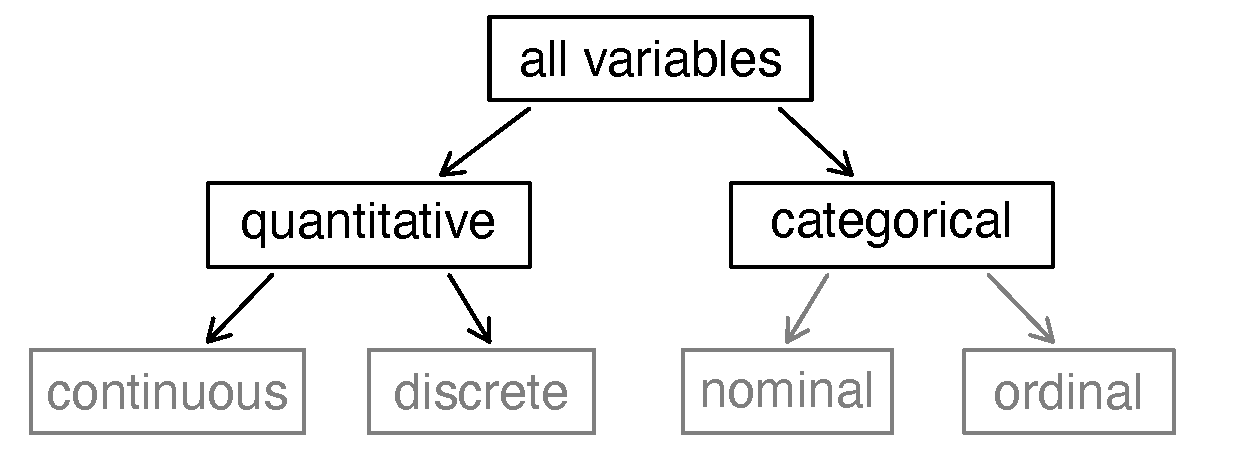
\includegraphics{images/variables.png}

\begin{enumerate}
\def\labelenumi{\arabic{enumi}.}
\setcounter{enumi}{2}
\tightlist
\item
  Identify the variable we are collecting on each observational unit in this study. What are we measuring on each student?
\end{enumerate}

\vspace{1in}

It is important to note that a variable is different than a summary statistic. A variable is measured on a \textbf{single observational unit} while a summary statistic is calculated from a group of observational units. For example, the variable \textbf{whether or not a student is considered in-state} can be measured on each individual student. In a class of 50 students we can calculate the proportion of students who are considered in-state, the summary statistic. Make sure you wrote the variable in question 3 as a variable \textbf{NOT} a summary statistic.

\begin{enumerate}
\def\labelenumi{\arabic{enumi}.}
\setcounter{enumi}{3}
\tightlist
\item
  Is the variable identified in question 3 categorical or quantitative?
\end{enumerate}

\vspace{0.5in}

\begin{enumerate}
\def\labelenumi{\arabic{enumi}.}
\setcounter{enumi}{4}
\tightlist
\item
  Were you correct or incorrect in identifying bumba?
\end{enumerate}

\vspace{0.5in}

We will now collect the data from the entire class.

\begin{enumerate}
\def\labelenumi{\arabic{enumi}.}
\setcounter{enumi}{5}
\tightlist
\item
  How many people in your class were correct in identifying bumba? Using the class size from question 2, calculate the proportion of students who correctly identified bumba.
\end{enumerate}

\begin{center}
$\mbox{proportion} = \frac{\mbox{number of students who correctly identified bumba}}{\mbox{total number of students}}$
\end{center}
\vspace{0.5in}

Looking at the data set and the summary statistics is only one way to display the data. We will also want to create a visualization or picture of the data. A \textbf{frequency bar plot} is used to display categorical data as a count or frequency. Since our variable has two levels, correct or incorrect, we will create two bars one for each level.

\begin{enumerate}
\def\labelenumi{\arabic{enumi}.}
\setcounter{enumi}{6}
\tightlist
\item
  Plot the observed class data using a frequency bar plot.
\end{enumerate}

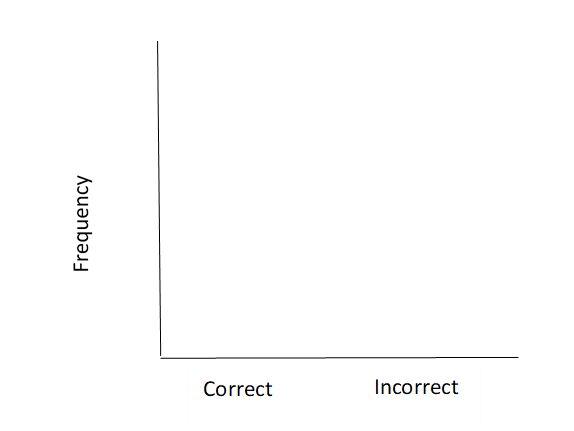
\includegraphics{images/barplot_martian.png}
\newpage 

We can also visualize the data as a proportion in a \textbf{relative frequency bar plot}. Relative frequency is the proportion calculated for each level of the categorical variable.

\begin{enumerate}
\def\labelenumi{\arabic{enumi}.}
\setcounter{enumi}{7}
\tightlist
\item
  Plot the observed class data using a relative frequency bar plot.
\end{enumerate}

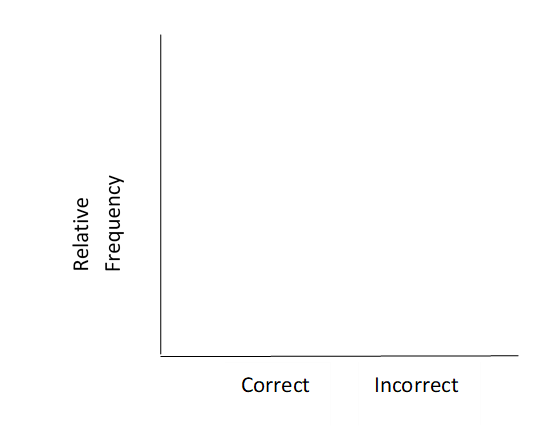
\includegraphics{images/relative_barplot_martian.png}

\begin{enumerate}
\def\labelenumi{\arabic{enumi}.}
\setcounter{enumi}{8}
\tightlist
\item
  The next step is to analyze the data. If humans really don't know Martian and are just guessing which is bumba, what are the chances of getting it right?
  \vspace{0.5in}
\end{enumerate}

\begin{verbatim}
How could we use a coin to simulate each student “just guessing” which martian letter is bumba? 
\end{verbatim}

\vspace{1in}

\begin{verbatim}
How could we use coins to simulate the entire class “just guessing” which martian letter is bumba? 
\end{verbatim}

\vspace{1in}

\begin{verbatim}
How many people in your class would you expect to choose bumba correctly just by chance?  Explain your reasoning.
\end{verbatim}

\vspace{1in}

\begin{enumerate}
\def\labelenumi{\arabic{enumi}.}
\setcounter{enumi}{9}
\tightlist
\item
  Each of you will flip a coin one time to simulate your ``guess''. Let Heads = correct, Tails = incorrect. What was the result of your simulation? \vspace{1in}
\end{enumerate}

\begin{verbatim}
What was the result from your class’s simulation?  What proportion of students “guessed” correctly in the simulation?
\end{verbatim}

\vspace{1in}

\begin{enumerate}
\def\labelenumi{\arabic{enumi}.}
\setcounter{enumi}{10}
\tightlist
\item
  If students really don't know Martian and are just guessing which is bumba, which seems more unusual: the result from your class's \textbf{simulation} or the observed proportion of students in your class that were correct (this is your data from question 6)? Explain your reasoning.
\end{enumerate}

\vspace{1in}

\begin{enumerate}
\def\labelenumi{\arabic{enumi}.}
\setcounter{enumi}{11}
\tightlist
\item
  While your observed class data is likely far different from the simulated ``just-guessing'' class, comparing our class data to a single simulation does not seem to give enough information. The differences seen could just be due to that set of coin flips! Let's simulate another class. Each student should flip your coin again. What was the result from your class's second simulation? What proportion of students ``guessed'' correctly in the second simulation? Create a plot to compare the two simulated results with the observed class result.
\end{enumerate}

\vspace{1in}

\begin{enumerate}
\def\labelenumi{\arabic{enumi}.}
\setcounter{enumi}{12}
\tightlist
\item
  We still unfortunately only have a couple of simulations to compare our class data to. It would be much better to be able to see how our class compared to hundreds or thousands of ``just-guessing'' classes. Since we don't want to flip coins all class period, your instructor will use a computer simulation to get 1000 trials. Fill in the following blanks to describe how we would create a simulation of random guessing with 1000 trials.
  \vspace{0.1in}
\end{enumerate}

\begin{verbatim}
Probability of correct guesses: _____
\end{verbatim}

\vspace{0.1in}

\begin{verbatim}
Sample size: _____
\end{verbatim}

\vspace{0.1in}

\begin{verbatim}
Number of repetitions: _____
\end{verbatim}

\vspace{0.1in}

\begin{enumerate}
\def\labelenumi{\arabic{enumi}.}
\setcounter{enumi}{13}
\tightlist
\item
  Sketch the distribution displayed by your instructor here, being sure to label each axis appropriately.
\end{enumerate}

\vspace{2in}

\begin{enumerate}
\def\labelenumi{\arabic{enumi}.}
\setcounter{enumi}{14}
\tightlist
\item
  Is your class particularly good or bad at Martian? How can you use the plot in question 14 to tell?
\end{enumerate}

\vspace{1in}

\begin{enumerate}
\def\labelenumi{\arabic{enumi}.}
\setcounter{enumi}{15}
\tightlist
\item
  Is it possible that we could see our class results just by chance if everyone was just guessing? Explain your reasoning.
\end{enumerate}

\vspace{1in}

\begin{enumerate}
\def\labelenumi{\arabic{enumi}.}
\setcounter{enumi}{16}
\tightlist
\item
  Is it likely that we could see our class results just by chance if everyone was just guessing? Explain your reasoning.
\end{enumerate}

\vspace{1in}

\begin{enumerate}
\def\labelenumi{\arabic{enumi}.}
\setcounter{enumi}{17}
\tightlist
\item
  Does this activity provide strong evidence that students were not just guessing at random? If so, what do you think is going on here? Can we as a class read Martian?
\end{enumerate}

\vspace{1in}

\textbf{Take Home Messages}

\begin{enumerate}
\def\labelenumi{\arabic{enumi}.}
\item
  In this course we will learn how to evaluate a claim by comparing observed results (classes' ``guesses'') to a distribution of many simulated results under an assumption like ``blind guessing.''
\item
  Blind guessing between two outcomes will be correct only about half the time. We can create data (via computer simulation) to fit the assumption of blind guessing.
\item
  Unusual observed results will make us doubt the assumptions used to create the simulated distribution. A large number of correct ``guesses'' is evidence that a person was not just blindly guessing.
\end{enumerate}

\hypertarget{statistical-investigations-for-two-categorical-variables}{%
\chapter{Statistical Investigations for Two Categorical Variables}\label{statistical-investigations-for-two-categorical-variables}}

Placeholder

\hypertarget{learning-objectives.}{%
\section{Learning Objectives.}\label{learning-objectives.}}

\hypertarget{terminology}{%
\section{Terminology}\label{terminology}}

\hypertarget{background}{%
\section{Background}\label{background}}

\hypertarget{vocabulary-review}{%
\section{Vocabulary Review}\label{vocabulary-review}}

\hypertarget{ask-a-research-question}{%
\section{Ask a Research Question}\label{ask-a-research-question}}

\hypertarget{summarize-and-visualize-the-data}{%
\section{Summarize and Visualize the data}\label{summarize-and-visualize-the-data}}

\hypertarget{use-statistical-analysis-methods-to-draw-inferences-from-the-data}{%
\section{Use statistical analysis methods to draw inferences from the data}\label{use-statistical-analysis-methods-to-draw-inferences-from-the-data}}

\hypertarget{types-of-errors}{%
\section{Types of Errors}\label{types-of-errors}}

\hypertarget{statistical-investigations-for-paired-data}{%
\chapter{Statistical Investigations for Paired Data}\label{statistical-investigations-for-paired-data}}

Placeholder

\hypertarget{learning-outcomes}{%
\section{Learning Outcomes}\label{learning-outcomes}}

\hypertarget{mean-difference-in-heart-rates-for-jumping-jacks-and-bicycle-kicks}{%
\section{Mean Difference in Heart Rates for Jumping Jacks and Bicycle Kicks}\label{mean-difference-in-heart-rates-for-jumping-jacks-and-bicycle-kicks}}

\hypertarget{review}{%
\section{Review}\label{review}}

\hypertarget{ask-a-research-question}{%
\section{Ask a Research Question}\label{ask-a-research-question}}

\hypertarget{summarize-and-visualize-the-data}{%
\section{Summarize and Visualize the Data}\label{summarize-and-visualize-the-data}}

\hypertarget{use-statistical-inferential-methods-to-draw-inferences-from-the-data}{%
\section{Use statistical inferential methods to draw inferences from the data}\label{use-statistical-inferential-methods-to-draw-inferences-from-the-data}}

\hypertarget{communicate-the-results-and-answer-the-research-question.}{%
\section{Communicate the results and answer the research question.}\label{communicate-the-results-and-answer-the-research-question.}}

\hypertarget{revisit-and-look-forward}{%
\section{Revisit and Look Forward}\label{revisit-and-look-forward}}

\end{document}
